\documentclass{resume}

\usepackage{xcolor}
\begin{document}

% new command defined ---------------------------------------------
\newcommand\tab[1][1cm]{\hspace*{#1}}
\newcommand\tob[1][0.2cm]{\hspace*{#1}}
\newcommand\tub[1][0.3cm]{\hspace*{#1}}
\fontfamily{ppl}\selectfont
%\colorlet{Mycolor1}{green!50!blue!50!}
\definecolor{lightblue}{RGB}{0, 150, 180}
\definecolor{emphblue}{RGB}{0, 120, 150}
\definecolor{turkishgreen}{RGB}{42,185,147}
\colorlet{emphblue}{turkishgreen}
\colorlet{fillheader}{turkishgreen}
% -----------------------------------------------------------------

% *************** PAGE - 1 ******************************************

% ======== INTRODUCTION PART ========================================

\noindent
% TOP general detais part ------------------------------------------
\begin{tabularx}{\linewidth}{@{}m{0.8\textwidth} m{0.2\textwidth}@{}}
{
	% 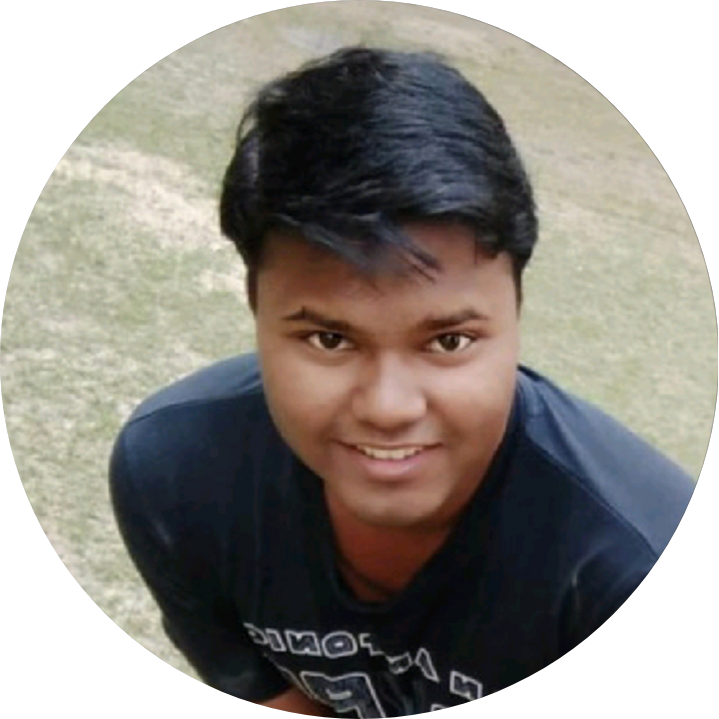
\includegraphics[width=0.6cm]{images/image3.png}
	\Large\textcolor{turkishgreen}{ \textbf{Akash Ramanand Rajak}} \newline
    \small{
        \clink{
            \href{mailto:aakashrajak02@gmail.com}{\textcolor{turkishgreen}{
\includegraphics[width=0.4cm]{images/mail.png}       \underline{aakashrajak02@gmail.com}}} \tob\textbf{|}\tob
            \href{mailto:435_bt19@iiitkalyani.ac.in}{\textcolor{turkishgreen}{
\includegraphics[width=0.4cm]{images/mail.png}       \underline{435\_ bt19@iiitkalyani.ac.in}}}
            \newline
            {
\includegraphics[width=0.4cm]{images/phone.png} \fontdimen2\font=0.75ex \textcolor{black}{+91 8980153352}}  \tob\textbf{|}\tob
            % \textbf{·} 
            %\href{https://johnmyweb.com}{johnmyweb.com}
        } % \newline
        
\includegraphics[width=0.4cm]{images/calender.png}
        \textcolor{black}{D.O.B.\tob :\tob 22\tob Nov,\tob 1999}
        \newline
        
\includegraphics[width=0.4cm]{images/location.png}
        \textcolor{black}{Gujarat,\tob India\tob  -\tob  391410}
    }
}
% ------------------------------------------------------------------

 & 

% Image Part ------------------------------------------------------
{
    \hfill
    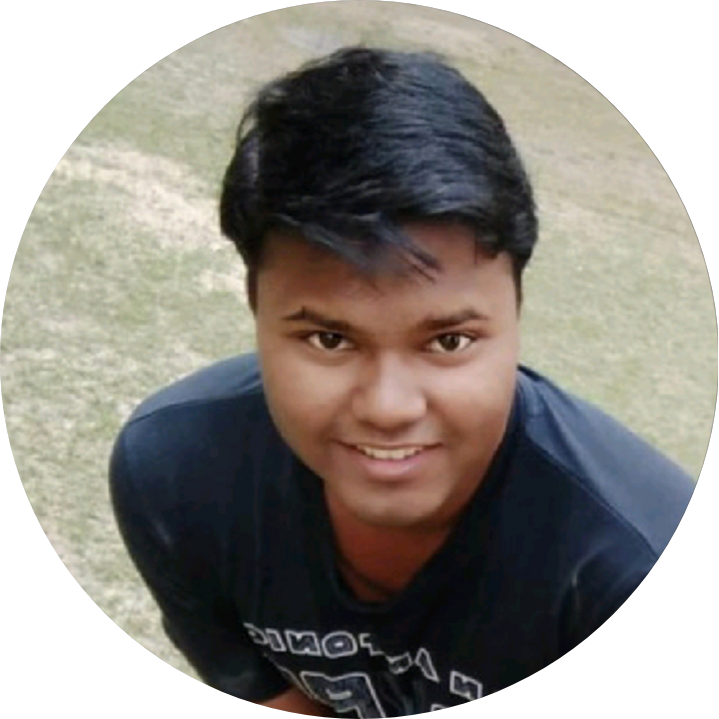
\includegraphics[width=3.0cm]{images/image3.png}
}
% -----------------------------------------------------------------
\end{tabularx}

% ===================================================================


\begin{center}
\begin{tabularx}{\linewidth}{@{}*{2}{X}@{}}
% left side %
{
	% -------- EDUCATION PART ----------------------------------
	\csection{\textcolor{turkishgreen}{EDUCATION}}{\small
        \begin{itemize}
        \item \frcontent{\textcolor{black}{B - Tech Computer Science  \tab \tob 2019 - 2023}}{}{}{Indian Institute of Information Technology, Kalyani\newline CGPA Till Sem - 4\tob :\tob 8.88}
            
            \item \frcontent{\textcolor{black}{HSC - Maths,Physics,Chemistry \tob 2016 - 2018}}{}{}{Baroda High School, Alkapuri \tab\tab\tob\tub 92.06 \%ile}
            
            \item \frcontent{\textcolor{black}{SSC \tab\tab\tab\tab\tab\tob\tub 2015 - 2016}}{}{}{Gujarat Refinery English Medium School\tub\tub\tob 98.95 \%ile}
        \end{itemize}
    }   
    
    % -------- EXPERIENCE PART ----------------------------------
   	\csection{\textcolor{turkishgreen}{EXPERIENCE}}{\small
        \begin{itemize}
            \item \frcontent{\textcolor{black}{Software Developer - Intern}}{Exposys Data Labs}{-\tob Project\tob :\tob Built an algorithm to secure messages with high security and less time. And also authenticated user entity.}{\tob  JUL 2021 - Aug 2021\tob (1 mos)}
        \end{itemize}
        \begin{itemize}
            \item \frcontent{\textcolor{black}{LGM SOC'21 - Open Source Contributor}}{Lets Grow More}{}{\tob  JUN 2021 - AUG 2021\tob (3 mos)}
        \end{itemize}
    }
    %\csection{\textcolor{turkishgreen}{}}{\small
        \small \begin{itemize}
            \item \frcontent{\textcolor{black}{Winter Of Code'21 - Student Member}}{Developer Student Club - IIIT Kalyani}{-\tob Project\tob :\tob Tabular ML (Built an end-to-end ML system for tabular datasets).\newline -\tob  Participated in Android Study Jam.}{\tob  JAN 2021 - MAR 2021\tob (3 mos)}
        \end{itemize}
    %}
    
    % -------- SKILLS PART ----------------------------------
	\csection{\textcolor{turkishgreen}{SKILLS}}{\small
        \begin{itemize}
        	\item \textbf{\textcolor{black}{Programming Languages \tob\&\tob Technologies}} \newline
            {\footnotesize - \tob C, C++, Java, Python, HTML-CSS, Scilab, MIPS \newline - \tob Dev C++, Pycharm, Jupiter Notebook, Eclipse,  Android Studio, Scilab, Qtspim, Git \& Github}{}{}
            \item \textbf{\textcolor{black}{Patterns \tob\&\tob Practices}} \newline
            {\footnotesize Problem Solving, ML/DL/NLP Model Creation}{}{}
            
            \item \textbf{\textcolor{black}{Languages}} \newline
            {\footnotesize English,  Hindi,  Gujarati}
        \end{itemize}
    } 
    
} 
% end left side %
& 
% right side %
{

    % -------- PROJECTS PART ----------------------------------
    \csection{\textcolor{turkishgreen}{PROJECTS}}{\small
        \begin{itemize}
            % PROJECT - 1 ----------------
            \item \frcontent{\textcolor{black}{CaveMan\tob -\tob The\tob Saviour} \clink{\href{https://github.com/akash435/CaveMan-The_Saviour}{\tob \textcolor{turkishgreen}{\underline{[Github\tob Link]}}}}}{-\tob A 2D physics - based flash game app created using ANDROID STUDIO and with simple graphics.}{}{+\tob Features used - Java, Android, Sqlite database}
            
			% PROJECT - 2 ----------------
            \item \frcontent{\textcolor{black}{Real Time Human Detection \& Counting} \clink{\href{https://github.com/akash435/Real-Time-Human-Detection-Counting}{\tob \textcolor{turkishgreen}{\underline{[Github\tob Link]}}}}}{-\tob A Python script to detect and count humans in real time images, videos \& through camera.}{}{+\tob Features used - Python (Tensorflow, OpenCv)}            
            
            % PROJECT - 2 ----------------
            %\item \frcontent{\textcolor{black}{Organ-Donors-Prediction} \clink{\href{https://github.com/akash435/Organ-Donors-Prediction}{\tob \textcolor{turkishgreen}{\underline{[Github\tob Link]}}}}}{-\tob Built a ML MODEL, to analyze the data of donors and predict from that. Analyzed with models like Logistic, Linear, Ridge, Lasso Regression, Decision Tree, Random Forest, K Neighbors, XGBoost Classifier.}{}{+\tob Features used - Python(Numpy, Pandas, Seaborn, matplotlib, sklearn), Regression, Classifier, Jupiter Notebook}
            % PROJECT - 3 ----------------
            %\item \frcontent{\textcolor{violet}{Crop-Fertilizers-Analysis-Prediction} \clink{\href{https://github.com/akash435/Crop-Fertilizers-Analysis-and-Prediction}{\tob \textcolor{turkishgreen}{\underline{[Github\tob Link]}}}}}{-\tob Built a ML model, to analyze the data of crop fertilizers and predict the fertilizers for crops. Analyzed with models like Logistic, Linear, Ridge, Lasso Regression, Decision Tree, Random Forest, K Neighbors.}{}{+\tob Features used - Python(Numpy, Pandas, Seaborn, matplotlib, sklearn), Regression, Classifier, Jupiter Notebook}
            
            % PROJECT - 3 ----------------
            \item \frcontent{\textcolor{black}{Video Stitching} \clink{\href{https://github.com/akash435/Video-Stitching}{\tob \textcolor{turkishgreen}{\underline{[Github\tob Link]}}}}}{-\tob Built a Video Stitching application with ROW and COLUMN STITCHING.}{}{+\tob Features used - Python (tkinter, opencv, moviepy, PIL)}
            
            % PROJECT - 4 ----------------
            \item \frcontent{\textcolor{black}{Dictionary} \clink{\href{https://github.com/akash435/Dictionary}{\tob \textcolor{turkishgreen}{\underline{[Github\tob Link]}}}}}{-\tob Built an English dictionary with AUTO-COMPLETE, TEXT - SPEECH, SPEECH - TEXT, VIRTUAL KEYPAD feature.}{}{+\tob Features used - Python (tkinter, pyttsx3, speech recognition, pyaudio)}
            
            % PROJECT - 5 ----------------
            \item \frcontent{\textcolor{black}{Simple Python IDE} \clink{\href{https://github.com/akash435/Simple-Python-IDE}{\tob \textcolor{turkishgreen}{\underline{[Github\tob Link]}}}}}{-\tob Built a  Simple Python IDE using tkinter GUI which runs code, find errors, change themes.}{}{+\tob Features used - Python (Tkinter, StringIO)}
        \end{itemize}
    }
    
    % -------- CERTIFICATIONS & AWARDS PART ----------------------------------
    \csection{\textcolor{turkishgreen}{Certifications \& Awards}}{\small
    	\begin{itemize}
            \item 
            \clink{
        	\href{https://drive.google.com/file/d/19sIphTJwHFJKjJBrUikXmT5E2ctzIoL-/view}{\textcolor{turkishgreen}{\underline{Codacharya'21 - 2nd Prize Winner}}}
        }
        \end{itemize}
        \begin{itemize}
            \item 
            \clink{
        	\href{https://drive.google.com/file/d/10sXwmb6wxSuvKRxmuy-zUPSzIliKLoce/view}{\textcolor{turkishgreen}{\underline{Code Kaze'21}}}
        	\textbf{|}
        	\href{https://drive.google.com/file/d/1yKLWfopv5k2C1YMbC8GmZNl1wXWj2vXq/view}{\textcolor{turkishgreen}{\underline{Code Frenzy}}}
        	\textbf{|}
        	\href{https://drive.google.com/file/d/19awkeMAFD8j4_Z2dlzMNZ6S2NCeMaOla/view}{\textcolor{turkishgreen}{\underline{LGM SOC'21}}}
        }
        \end{itemize}
        
        \begin{itemize}
            \item 
            \clink{
        	\href{https://drive.google.com/file/d/11pssUHnwQSHhpv3muc3RsOlsujGNo9Zt/view}{\textcolor{turkishgreen}{\underline{Android Study Jam}}}
        	\textbf{|} 
        	\href{https://drive.google.com/file/d/1LdR-E4uXdbXYD3yLiHGOtKpeYbjZcNo6/view}{\textcolor{turkishgreen}{\underline{GDSC -  Winter Of Code}}}
        }
        \end{itemize}
        \begin{itemize}
            \item 
            \clink{
        	\href{https://www.udemy.com/certificate/UC-05ceea42-245e-46fc-a343-d30bfbf2baef/}{\textcolor{turkishgreen}{\underline{Udemy - NLP Basic Course}}}
        	\newline
        	\href{https://www.udemy.com/certificate/UC-e7b09c62-176d-42c1-903a-29c8799b87a5/}{\textcolor{turkishgreen}{\underline{Udemy - Complete Python \& OOPs Course}}}
        }
        \end{itemize}
        \begin{itemize}
            \item 
            \clink{
        	\href{https://www.credential.net/42a575f4-de1e-45b6-87e8-7dadd16bfe11}{\textcolor{turkishgreen}{\underline{Pirple - Frontend Fundamentals}}}
        }
        \end{itemize}
    }
    
}
\end{tabularx}
\end{center}
% ********************************************************************

% *************** PAGE - 2 ******************************************

\begin{center}
\begin{tabularx}{\linewidth}{@{}*{2}{X}@{}}
% left side %
{
    % -------- COURSES PART ----------------------------------
    \csection{\textcolor{turkishgreen}{COURSES}}{\small
        \begin{itemize}
            \item \textbf{\textcolor{black}{Mathematics}} \newline
            {\footnotesize Linear Algebra, Probability \& Statistics, Discrete Mathematics, Calculus \& Differential Equation, Numerical Analysis \& Computing, Computational Number Theory}{}{}
            \item \textbf{\textcolor{black}{Computer Science}} \newline
            {\footnotesize Programming with C, Data Structures \& Algorithm, Algorithm Analysis \& Design, Computer Architecture, Formal Language \& Automata Theory, Data Science (Python), Operating System, Object Oriented Programming (JAVA), Scilab, Qtspim, Compiler Design, Artificial Intelligence}
            \item \textbf{\textcolor{black}{Electronics}} \newline
            {\footnotesize Digital Electronics, Analog Electronics, Data Communication, Signals \& Systems, Microprocessor \& Microcontroller System}
            \item \textbf{\textcolor{black}{Others}} \newline
            {\footnotesize Physics, Ethics, Economics, Humanity (Psychology)}
        \end{itemize}
    }
    
    % ------------ Interest and Hobbies section ---------------
    \csection{\textcolor{turkishgreen}{Interests \& Hobbies}}{\small
        \begin{itemize}
            \item {\footnotesize Competitive Programming\tab \textbf{•} \tob Open Sourcing}
        \end{itemize}
    }
    
} 
% end left side %
& 
% right side %
{
	% -------- EVENTS & PARTICIPATIONS PART ----------------------------------
    \csection{\textcolor{turkishgreen}{Events \& Participations}}{\small
        \begin{itemize}
            \item {\footnotesize Google Coding Competition 2021, Facebook HackerCup 2021.}
            \item {\footnotesize Devfolio Hackathon HackData 5.0, with project BSM.}
            \item {\footnotesize Code Kaze'21, Code Frenzy - Online Coding Competion by Coding Ninjas.}
            \item {\footnotesize Codacharya 2021 - 4th Annual Coding Competition organized by IIIT Kalyani.}
        \end{itemize}
    }
   
    % -------- LINKS PART ----------------------------------
	\csection{\textcolor{turkishgreen}{LINKS}}{\small
        \begin{itemize}
            \item 
            \clink{
        	\href{https://github.com/akash435}{\textcolor{turkishgreen}{
\includegraphics[width=0.4cm]{images/github.png}\tob   \underline{Github}}}
        	\textbf{} 
        	\href{https://www.linkedin.com/in/akash-rajak-akash435/}{\textcolor{turkishgreen}{
\includegraphics[width=0.4cm]{images/linkedin.png}\tob \underline{Linkedin}}}
        	\textbf{}
        	\href{https://www.hackerrank.com/aakashrajak02?hr_r=1}{\textcolor{turkishgreen}{
\includegraphics[width=0.4cm]{images/hackerrank.png}\tob \underline{HackerRank}}}
        }
        \end{itemize}
        
        \begin{itemize}
            \item 
            \clink{
        	\href{https://www.codechef.com/users/akash435}{\textcolor{turkishgreen}{
\includegraphics[width=0.4cm]{images/codechef.png}\tob \underline{CodeChef}}}
        	\textbf{}
        	\href{https://codeforces.com/profile/aakashrajak02}{\textcolor{turkishgreen}{
\includegraphics[width=0.4cm]{images/codeforces.png}\tob \underline{Codeforces}}}
        	\textbf{}
        	\href{https://leetcode.com/akash435/}{\textcolor{turkishgreen}{
\includegraphics[width=0.4cm]{images/leetcode.png}\tob \underline{LeetCode}}}
            %\newline
        }
        \end{itemize}
    }
}
\end{tabularx}
\end{center}

% *******************************************************************

\end{document}\
